% =========================================================================== %
% TeX input file: "Create a new project"
%
% WARNING: this tex file does not compile standalone, it needs to be embedded
% in a master tex document (e.g. Introduction.tex)
% =========================================================================== %

Start your Eclipse IDE and select an empty directory for your workspace.
This workspace directory will then hold all the project code for the ''Hello World'' application.
In the started Eclipse IDE, you can then create a new Scout project by selecting the \contextmenu{New Scout Project...} as shown in \figref{sdk_create_new_scout_project}.
Alternatively, you can also use the Eclipse \menu{File|New|Project...}.
In this case you are shown the generic \wizard{New Project} of Eclipse where you can select the \wizard{Scout Project} below the Scout folder as seen in \figref{sdk_new_project_wizard}.
With the \button{Next} you will be directed to the next dialog step, the \wizard{New Scout Project}.

\begin{figure}
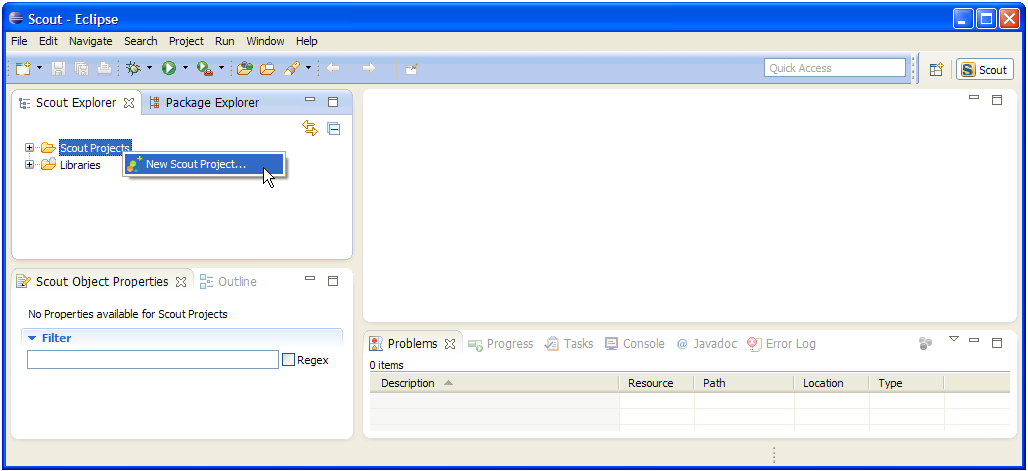
\includegraphics[width=15cm]{sdk_create_new_scout_project.png}
\caption{Create a new Scout project using the Scout SDK perspective.}
\figlabel{sdk_create_new_scout_project}
\end{figure}

In the \wizard{New Scout Project} enter a name for you Scout project. 
As we are creating a ''Hello World'' application, use \java{org.eclipsescout.helloworld} for the \field{Project Name}.
Now, click the \button{Finish} to let the Scout SDK create the initial project code for you.

\begin{figure}
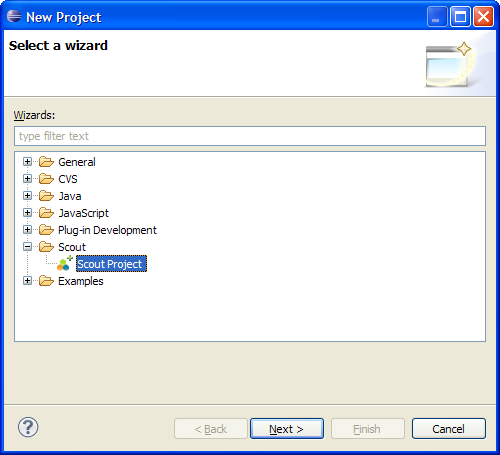
\includegraphics[width=7cm]{sdk_new_project_1.png} \hspace{5mm}
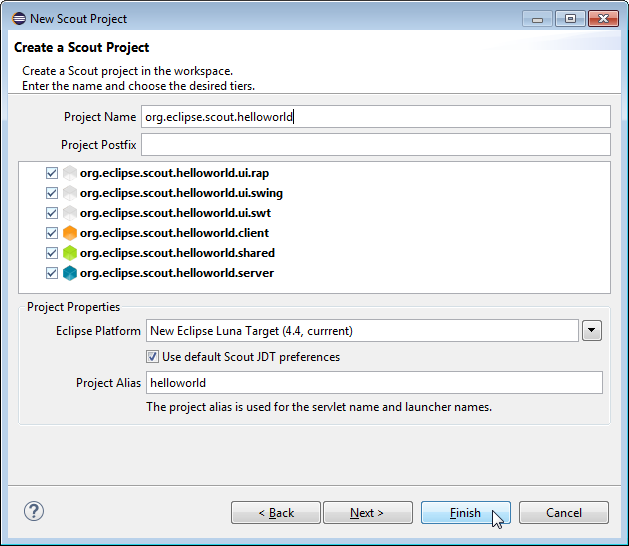
\includegraphics[width=7cm]{sdk_new_project_2.png}
\caption{The new project wizard. The dialog on the left side is only shown when using the generic \wizard{New Project} of Eclipse}
\index{SDK Wizard!New Scout Project}
\figlabel{sdk_new_project_wizard}
\end{figure}

\begin{figure}
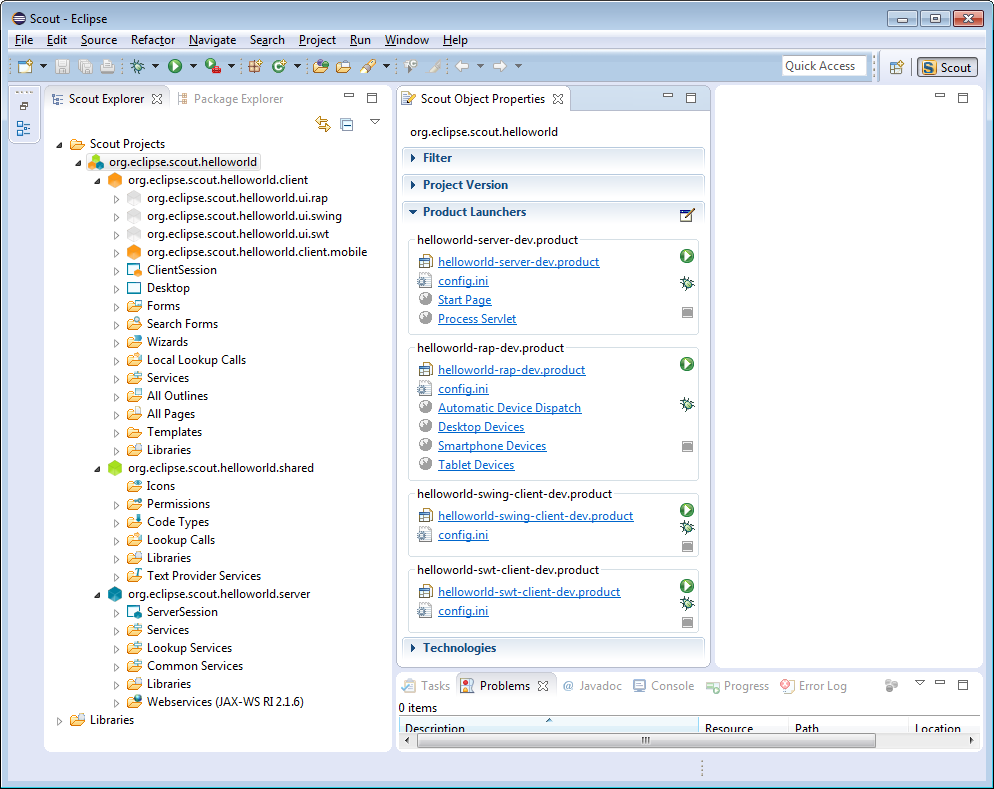
\includegraphics[width=15cm]{sdk_initial_helloworld_project.png}
\caption{The Scout SDK showing the tree representation of our ''Hello World'' application in the Scout Explorer.
Scout Object Properties displays the product launchers for the server and the available clients.}
\figlabel{sdk_initial_helloworld_project}
\end{figure}

Once the initial project code is built, the Scout SDK displays the application model in the \textit{Scout Explorer}.
This model is visually presented as a tree structure covering both the client and the server part of the application.
In \figref{sdk_initial_helloworld_project} the Scout Explorer displays the top level elements of the complete Scout application.

% =========================================================================== %
% EOF TeX input file
% =========================================================================== %
